\documentclass{beamer}
\usetheme{metropolis} 
\title{\huge Konobi}
\date{}
\subtitle{Software Development Methods project}
\author{Lorenzo Basile, Irene Brugnara, Roberto Corti, Arianna Tasciotti}
\usepackage{caption}
\begin{document}
  \maketitle
  \section{Introduction}
  \begin{frame}{Our project}
    The goal of our project was to develop a command line version of \textbf{Konobi}, a board game for two players. The project also contains a client-server version of the game.
    \vspace{0.7cm}
    \pause
    \\What tools did we use?
    \begin{itemize}
    \item Java 15
    \item Gradle
    \item TravisCI
    \item Git \& GitHub
    \end{itemize}
    \end{frame}
  \begin{frame}{Konobi}
    Konobi is a drawless game and it can be played either on a go board or a chess board.
    \\Two players, black and white, take turns at placing stones of their color on the board, starting with black. The aim of the players is to build chains of connected stones of their color.
    \vspace{0.5cm}
    \pause
    \\The game is won by the first player who connects the two opposite edges of the board.
    \begin{itemize}
    \item Black: top $\leftrightarrow$ bottom
    \item White: left $\leftrightarrow$ right
    \end{itemize}
      \end{frame}
      
     \begin{frame}{Connections}
     Two like-colored stones are:
     \vspace{0.5cm}
    \begin{columns}
			\column{0.5\textwidth}
			\begin{figure}
				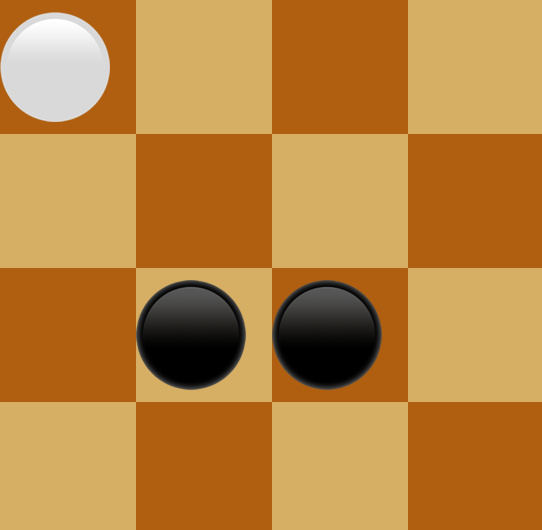
\includegraphics[scale=0.35]{images/strong.png}
				\caption*{Strongly connected}
			\end{figure}
					
			\column{0.5\textwidth}
			\begin{figure}
				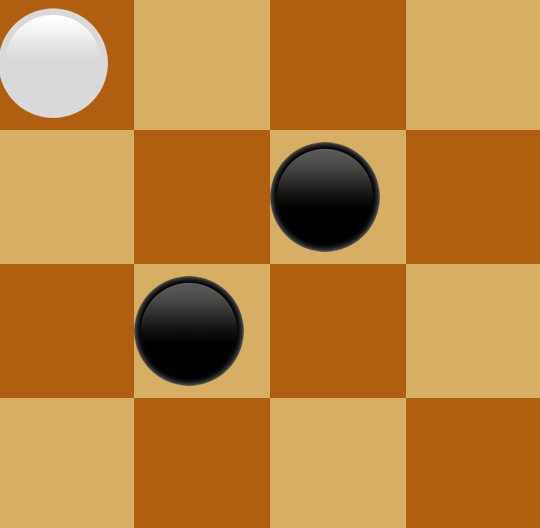
\includegraphics[scale=0.35]{images/weak.png}
				\caption*{Weakly connected}
			\end{figure}
		
	\end{columns}
	\vspace{0.7cm}
	A chain is a set of connected stones

      \end{frame}
      
      \begin{frame}{Placement rules}
     Not all moves are allowed:
     \begin{itemize}
     \item \textbf{Weak connections} to a certain stone are illegal unless it is impossible to make a placement that is both strongly connected to that stone and not weakly connected to another
     \item \textbf{Crosscut} placements are always illegal
     \end{itemize}
    \begin{columns}
			\column{0.5\textwidth}
			\begin{figure}
				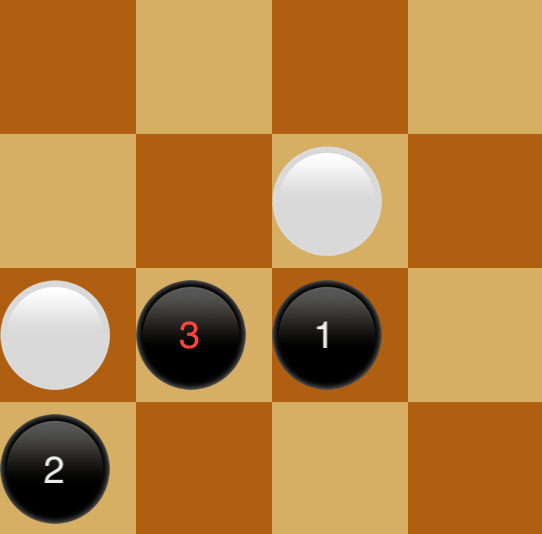
\includegraphics[scale=0.35]{images/legal_weak.png}
				\caption*{Legal weak connection}
			\end{figure}
					
			\column{0.5\textwidth}
			\begin{figure}
				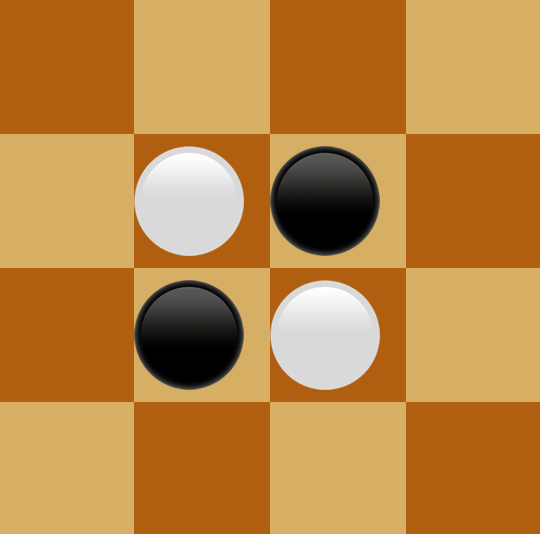
\includegraphics[scale=0.35]{images/crosscut.png}
				\caption*{Crosscut placement}
			\end{figure}
		
	\end{columns}
      \end{frame}
      
      \begin{frame}{Additional rules}
     \begin{itemize}
     \item \textbf{Pie rule}: at his first move, white can decide to switch colors with black instead of making a move
     \item \textbf{Mandatory pass}: if a player cannot make a move (because of placement restrictions), he has to pass
     \end{itemize}
      \end{frame}
      
      
\section{Basic entities}
\begin{frame}{Cell}
% Lorenzo parla dei pacchetti
% inizio a parlare delle classi color, position, cell, board (diagramma uml)

\begin{columns}
\column{0.5\textwidth}
\texttt{Cell} represents the basic building block of the board 
% A cell has three fields: the position of the cell in the board, a boolean isOccupied which tells whether the cell contains a stone or not, and a Color which is the color of the stone if present.
\vspace{0.5cm}
\begin{itemize}
    \item \texttt{Position position }
    % position has two fields x,y
    \item \texttt{Color color}
    % color is an enum with two values BLACK, WHITE
    \item \texttt{boolean isOccupied}
    

    
\end{itemize}

\column{0.5\textwidth}
% uml con i tre data membri
\end{columns}

\vspace{0.5cm}
When a cell is constructed it is empty: no color is associated to it and \texttt{isOccupied=False}, when a stone is placed in the cell a color is set and \texttt{isOccupied=True}.

% The methods setColor() and reset() are used for checking the rules, as we will see later. For this reason, Color is not final, even if in the game once a stone is placed it cannot be moved afterwards. The position is final because a cell is associated with a fixed position in the board.


\end{frame}

\begin{frame}{Cell: development history}
\begin{itemize}
\item From value \texttt{NONE} in enum \texttt{Color} to field \texttt{isOccupied} in class \texttt{Cell}
\item Removed \texttt{Stone} data class
\end{itemize}
% At the beginning, the Color enum had also a NONE value, but then we thought that a Player cannot have NONE as a value for his color so we moved NONE into a new field of Cell which is a boolean called isOccupied, and the color can be only WHITE or BLACK, which is also more logical.
%When a cell is constructed it is empty, i.e. no Color is associated to it and isOccupied=False, when a stone is placed in the Cell a Color is given and isOccupied=True with the setColor() method.

% at the beginning we had a class Stone but we removed it because it was a data class (only had setters, ..) and it basically coincided with Color

\end{frame}


\begin{frame}{Board}

A \texttt{Board} is represented by a set of Cells and extends \texttt{HashSet<Cell>} by overriding the \texttt{dimension()} method
\begin{itemize}
    \item Usage of streams
    \item \texttt{Position} as field of \texttt{Cell}    
\end{itemize}



% The board is represented by a set of cells. The other option we considered was a 2-dimensional array. In this way we can easily use streams to perform operations on this set of cells (we will see with connections). And in addition, the Position is a property (a field) of a Cell and not a pair of indexes of a matrix.

The constructor of Board creates a set of empty cells

\end{frame}


\begin{frame}{Connections among cells}


\end{frame}
     
\end{document}